\documentclass{article}
\usepackage{amsfonts} % \mathbb
\usepackage[margin=0.5in]{geometry}
\usepackage[utf8]{inputenc}
\usepackage{graphicx} 

\title{Interference Transform: Estimating the frequency and phase of low resolution samples}
\author{
  Carlos Tarjano
  \and 
  Valdecy Pereira
  }

\begin{document}

\maketitle

\begin{abstract} % 250 words
  % background
  The Fourier Transform, naturally due to the context and time in which it was idealized, was formulated without regard to discrete waves or computational complexity.
  Some developments, such as the Discrete Fourier Transform and the Fast Fourier Transform algorithm updated the theory to the digital, discrete era.
  % motivation
  Some shortcomings were introduced with those methods, such as diminishing resolution in dealing with increasingly small number of os samples.
  % objective
  In this paper we propose a formal framework based on discrete waves, optimizing the inference of frequency and amplitude from whatever sampled points are available. Although arising from a intuitively different approach, the framework here presented can be viewed as a generalization of the Discrete Fourier Transform.
  % methods
  The algorithm is based on the representation of the set of samples in a frequency versus phase space and the investigation of the interference pattern thus generated. Each sample defines a sinusoidal planar wave in this space, with a particular amplitude, direction and frequency. The determination of the point in which maximum constructive interference occurs translates to the determination of the most accurate sinusoidal description of the whole set of samples.
  % results
  TODO: improvement of the naïve algorithm. better accuracy
  % implications
  TODO: an alternative to wavelet and short-time Fourier transform
\end{abstract}

{\bf Keywords:} Fast Fourier Transform, Digital Signal Processing, Wavelet Transform

\section{Introduction}

Despite the ubiquitous presence of the DFT algorithm, some of its shortcomings, specially with respect to low resolution waves, are yet to be addressed. Nevertheless, areas such as audio compression would greatly benefit from improved analysis of the characteristics of low resolution samples, enabling, for example, the extraction of parameters to be used in machine learning algorithms or sound restoration.

This neglect is felt in the virtual inexistence of research in this specific topic.  

\subsection{Literature Review}

\section{Methodology}

\subsection{Theory}
  One can represent the discrete wave as an an array $ W[i] $ of $ n-1 $ real numbers. Such wave is related, as illustrated in figure \ref{fig:ContinuousVsDiscrete}, to an hypothetical continuous wave $ S(t) $ of which its components are sampled in uniform time intervals at a rate of $\textrm{fps}$ frames per second.

  \begin{figure}[h!]
    \centering
      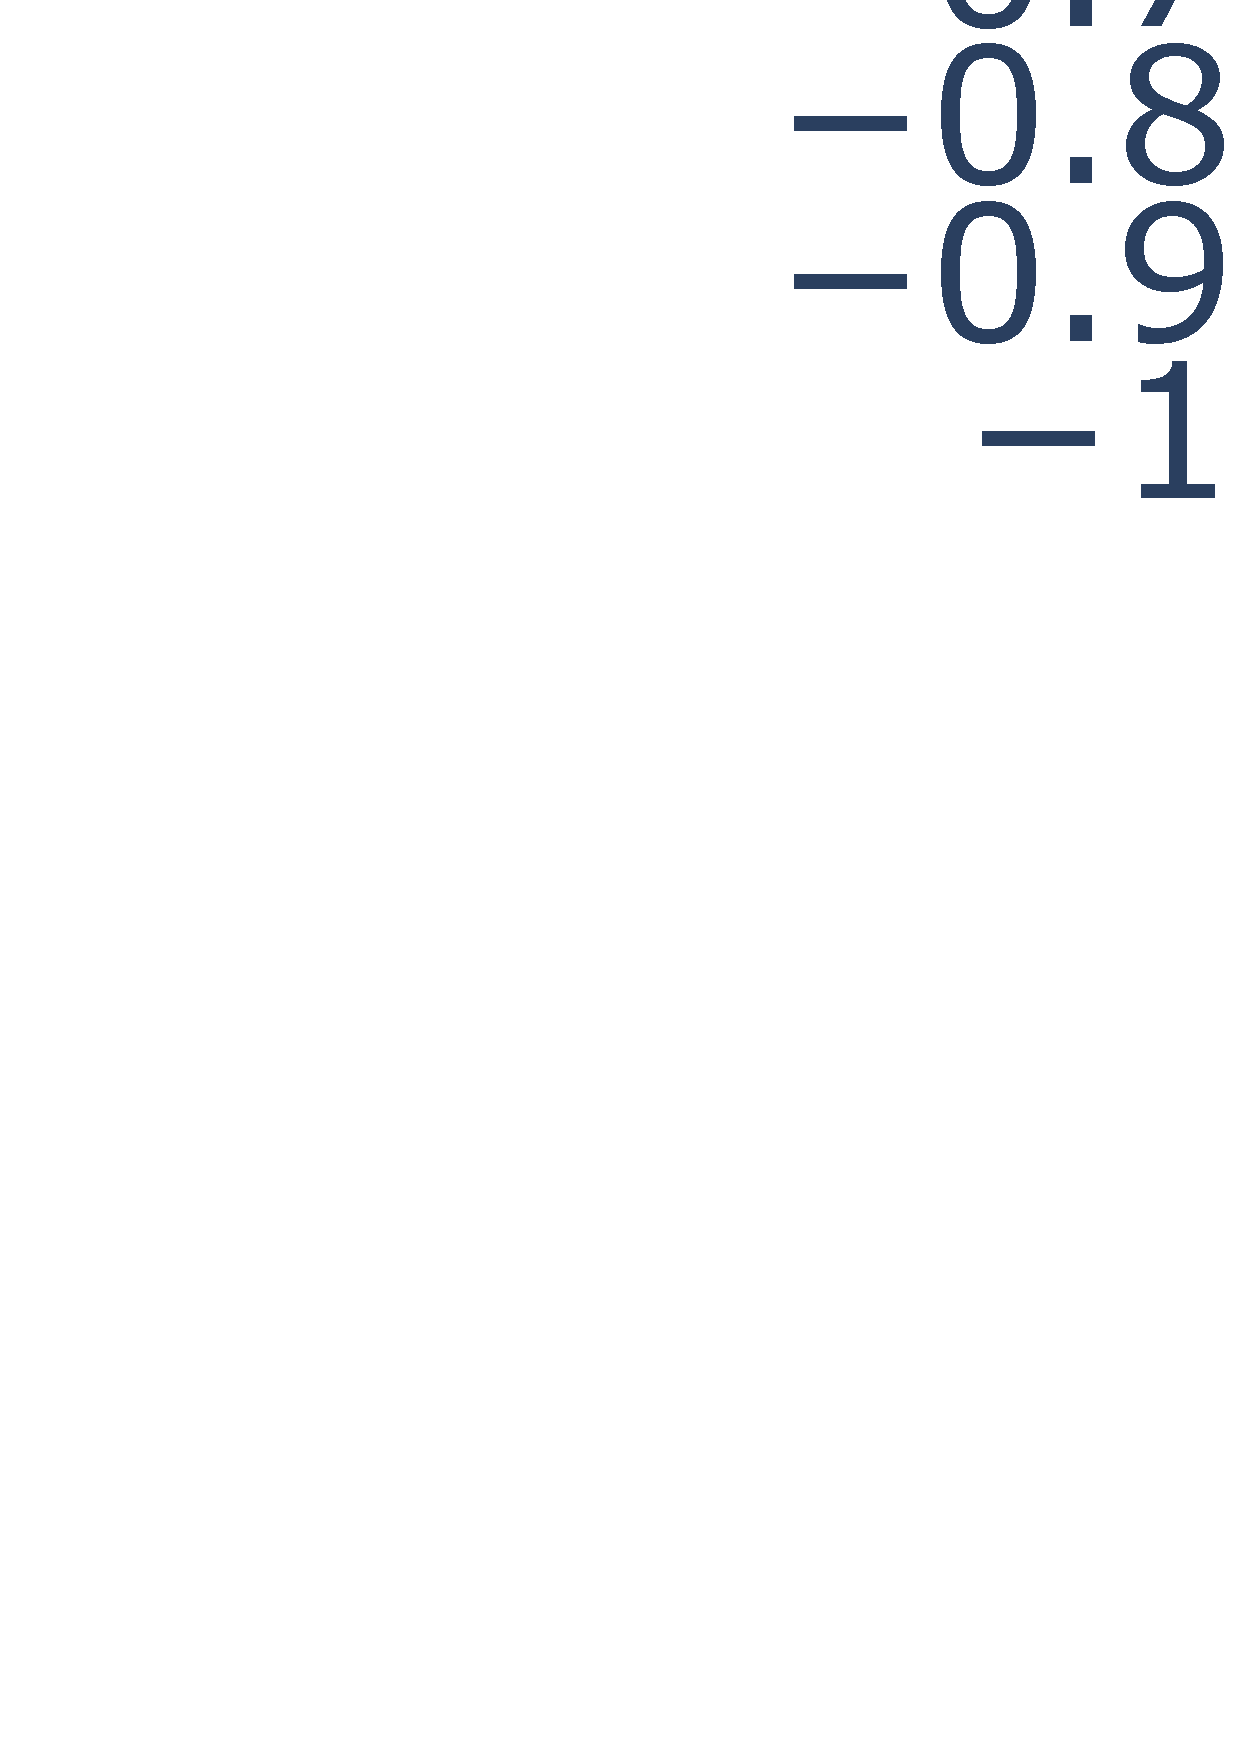
\includegraphics[width=0.8\linewidth]{images/01ContinuousVsDiscrete.pdf}
    \caption{Discrete samples (black points) from a continuous wave (grey line). Note that the amplitude is also truncated}
    \label{fig:ContinuousVsDiscrete}
  \end{figure}

  Thus, we have:
  $ W[i] \in \mathbb{R} \  \forall \  i \in \mathbb{N}, 0 \le i < n $
  $ S(t) \in \mathbb{R} \  \forall \  t \in \mathbb{R}, 0 \le t < t_f $ where $ t_f=\frac{n}{\textrm{fps}} $.

  The relationship is better illustrated comparing two equivalent simple sinusoids; a continuous one and its discrete counterpart. Those can be described, respectively as 
  $$ S(t) = a \cos \left( \phi + 2 \pi \mathcal{F} t \right) $$
  and
  $$ W[i] = a \cos \left( \phi + 2 \pi f \frac{i}{n} \right) $$
  where:

  $ \mathcal{F} \in \mathbb{R}^+ $, absolute frequency of the continuous wave in Hz;

  $ f \in \mathbb{R}^+ $, relative frequency of the discrete wave in cycles per $n$ samples;

  $ f = \frac{n}{\textrm{fps}} \mathcal{F} $;

  $ i = t \  \textrm{fps}, i \in \mathbb{N} $, frame number;

  $ t \in \mathbb{R} $, time in seconds;

  $ n \in \mathbb{N} $, number os discrete samples;

  $ 0 \le \frac{i}{n} < 1 $;

  $ a \in \mathbb{R}^+ $, amplitude;

  $ \phi \in \mathbb{R}^+, 0 \le \phi < 2 \pi $, phase; \\

  Figure \ref{fig:ContinuousVsDiscreteSinusoid} illustrates the relationship between the two.
  
  \begin{figure}[h!]
    \centering
      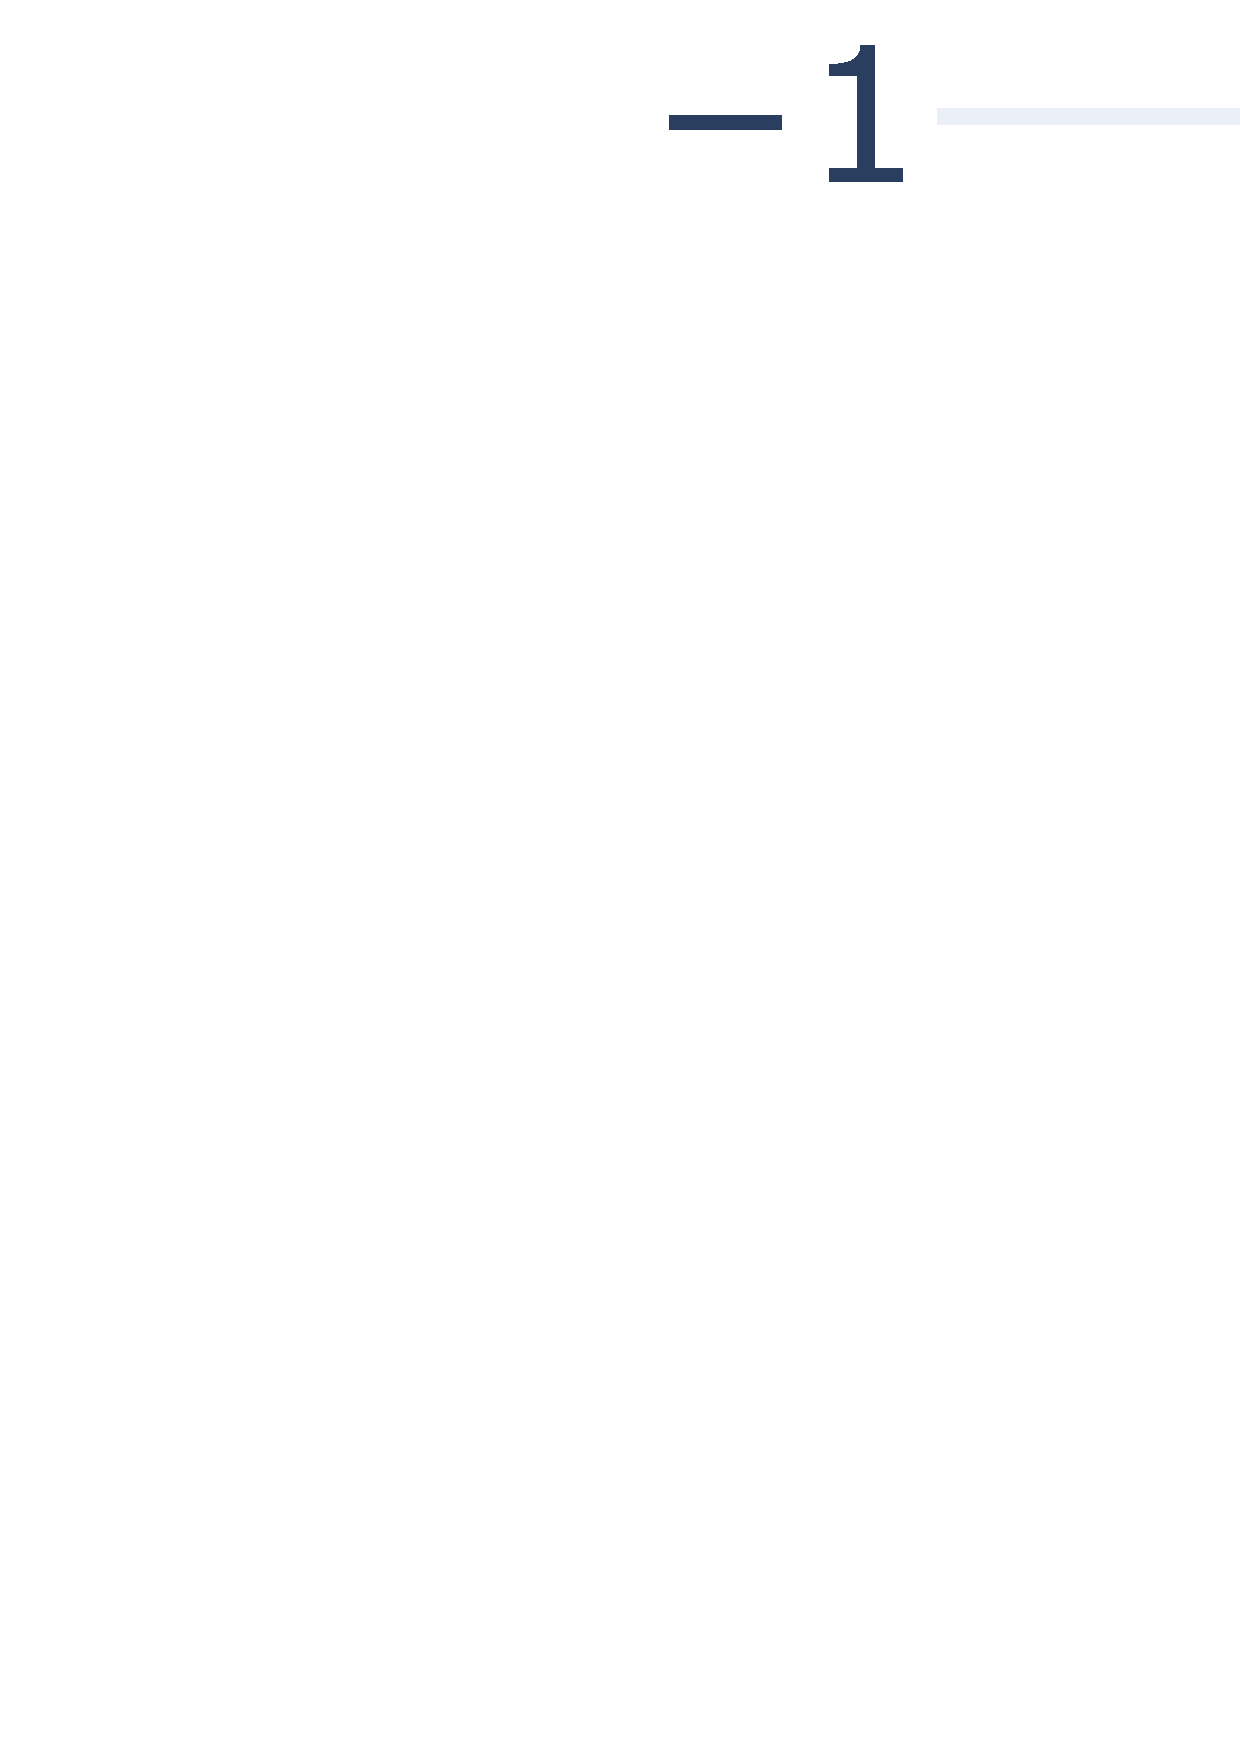
\includegraphics[width=0.8\linewidth]{images/02ContinuousVsDiscreteSinusoid.pdf}
    \caption{Continuous sinusoid (grey line) and the correspondent Discrete sinusoid (black points) illustrating the correspondence between frames i and time t}
    \label{fig:ContinuousVsDiscreteSinusoid}
  \end{figure}
  
  So it's easy to see that, for each frame of a given discrete wave $W[i]$, there exists an infinite family of continuous sinusoids that pass exactly through the point defined by $i$ and $W[i]$. In fact, almost any sinusoid of the form $a \cos \left( \phi + 2 \pi f \frac{i}{n} \right)$ can be forced to contain the point $(i, W[i])$, given a suitable choice of $a$, with the exception of the particular case where $W[i] \ne 0$ and $\cos \left( \phi + 2 \pi \mathcal{F} \frac{i}{\textrm{fps}} \right)$. 
  
  Of interest to this work are those sinusoids, as shown in Figure \ref{fig:OptSinusoids}, that have one of their infinite extrema, either maximum or minimum, coinciding with the abscissa $i$ or, setting $a=W[t]$, coincident with the point $(i, W[i])$.
  
  \begin{figure}[h!]
    \centering
      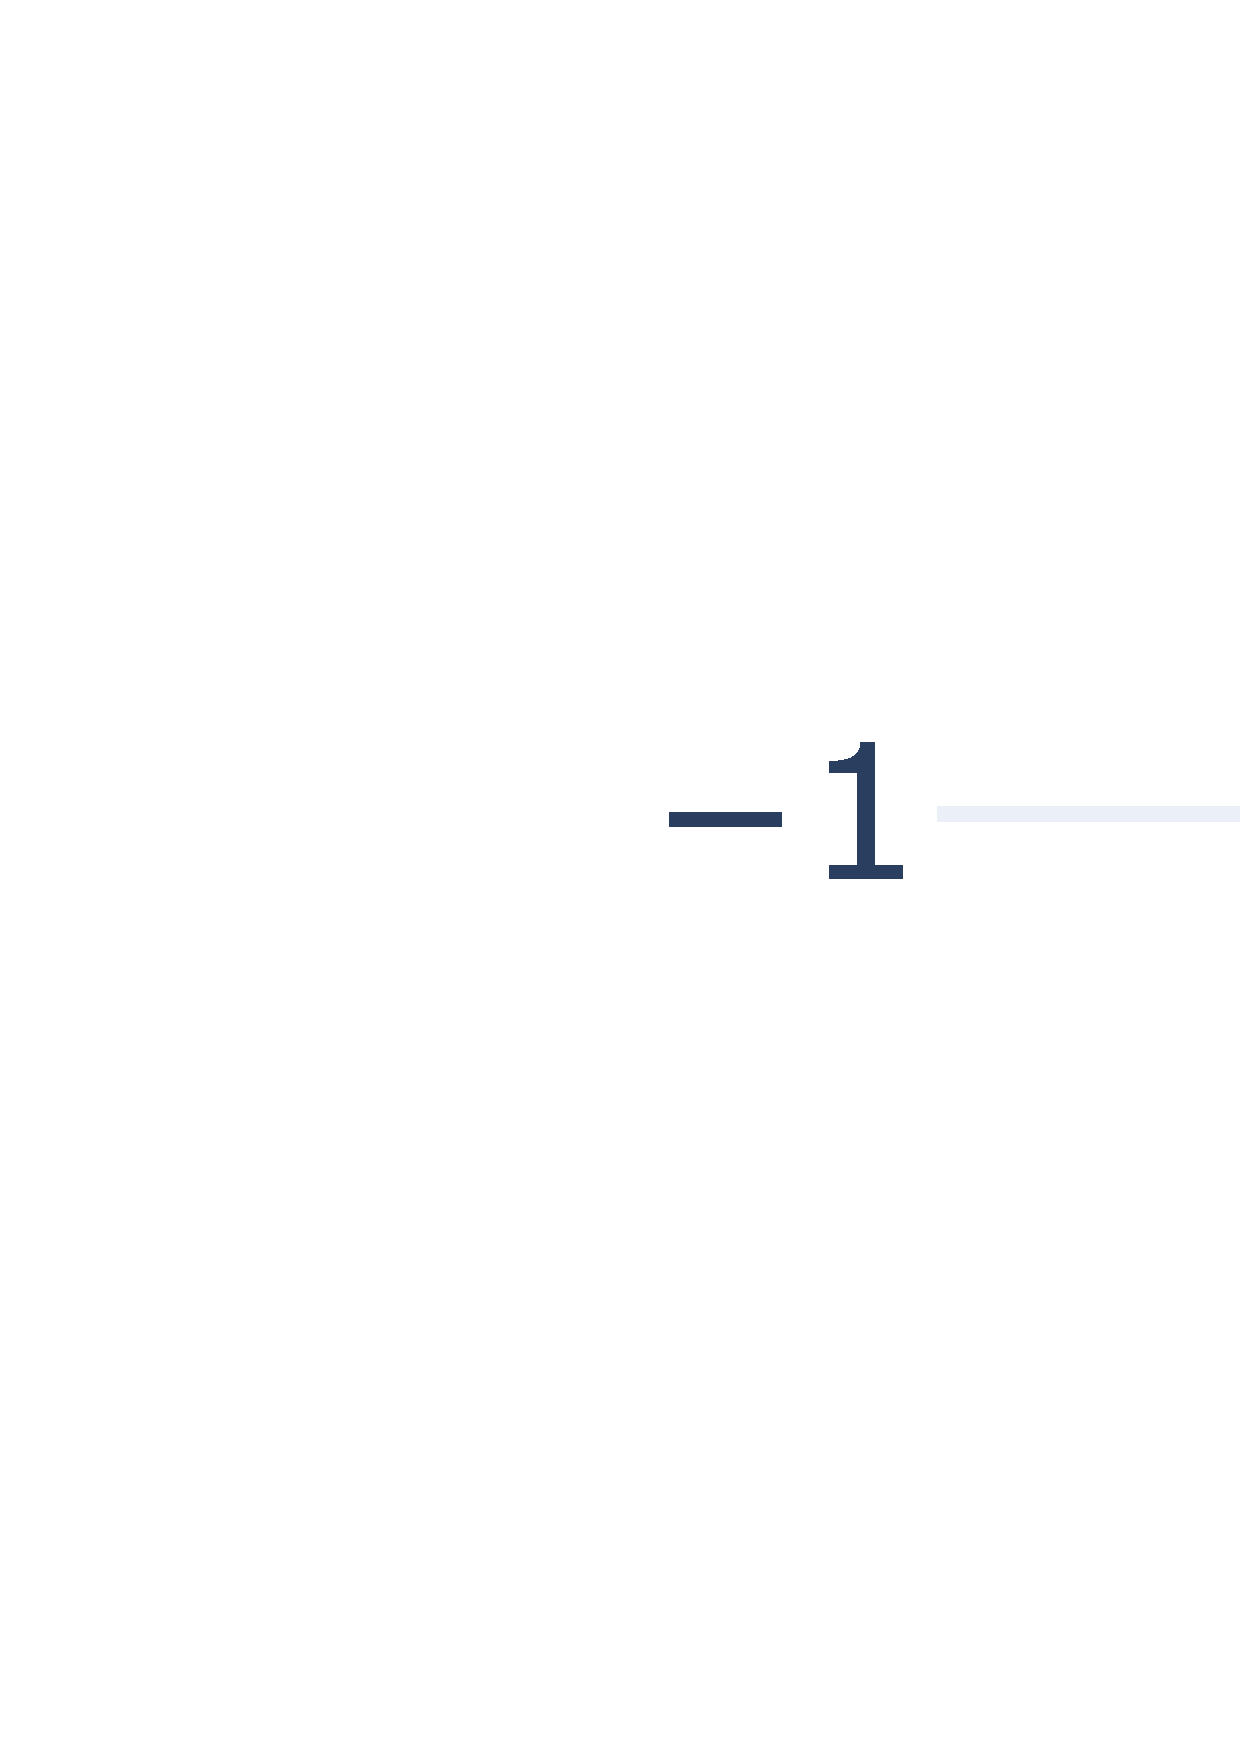
\includegraphics[width=0.8\linewidth]{images/03OptSinusoids.pdf}
    \caption{Sinusoids with maximum coinciding with frames i=3 and i=28 }
    \label{fig:OptSinusoids}
  \end{figure}

  One can define, for each frame, those waves mathematically as the family of continuous sinusoids that satisfy the equality $\cos \left( \phi + 2 \pi \mathcal{F} t \right) = \textrm{sgn}(W[t])$ or, in terms of discrete sinusoids, $\cos \left( \phi + 2 \pi f \frac{i}{n} \right) = \textrm{sgn}(W[t])$ where the sign function is defined as 
  $ \textrm{sgn}(x) = \{ -1 \  \textrm{if} \ x < 0, \  0  \  \textrm{if} \ x = 0, \  1  \  \textrm{if} \ x > 0\}$.



  
\section{Results}

\section{Discussion + Conclusion}

\section{References}

\end{document}
